%% ============================================================================
%% INCOM 2027 draft -- Learning disruption cascades in product-integrated
%% supply networks.
%%
%% Template: IFAC conference class (ifacconf.cls + ifacconf.bst), available
%% from the IFAC author kit. Place ifacconf.cls next to this file.
%%
%% NUMBERS IN RED (\pilot{...}) come from the notebook's MODE="quick" pilot
%% (33 small networks, one training seed). Replace every one of them with the
%% MODE="incom" results before submission. Figures in figures/ are exported
%% from the same pilot run of incom2027_cascade.ipynb.
%%
%% REFERENCES were written from memory -- verify every entry (authors, year,
%% volume, pages) before submission.
%% ============================================================================
\documentclass{ifacconf}

\usepackage{graphicx}
\usepackage{natbib}
\usepackage{amsmath,amssymb}
\usepackage{booktabs}
\usepackage{xcolor}
\usepackage{algorithm}
\usepackage{algpseudocode}
\usepackage{seqsplit}
\graphicspath{{figures/}}

\newcommand{\pilot}[1]{\textcolor{red}{#1}}   % pilot value: replace after the full run
\newcommand{\todo}[1]{\textcolor{red}{[#1]}}
\newcommand{\nbcommit}{c06c2f6064da}           % commit of the executed notebook
\newcommand{\netdigest}{\seqsplit{59909c87b96ba5f0bea045587b511f4e50c461982d1088a82eb4c07470125571}}       % pilot network digest (SHA-256)
\newcommand{\labeldigest}{\seqsplit{f4f87991e2450fcaba3774c17f898da5ff7dec33e016fa59b60ca089e52be15f}}   % pilot label digest (SHA-256)

\begin{document}
\begin{frontmatter}

\title{Learning Disruption Cascades in Product-Integrated Multi-Tier Supply Networks with Graph Neural Networks}

\author[First]{Phu Nguyen}
\author[Second]{\todo{Co-author}}

\address[First]{\todo{Affiliation, address} (e-mail: \todo{e-mail}).}
\address[Second]{\todo{Affiliation, address} (e-mail: \todo{e-mail}).}

\begin{abstract}
When a firm deep in a supply network fails, the damage travels further than its customers: alternative suppliers are overloaded by rerouted orders, and suppliers are hit by the order surge when the failed firm restarts. We study these cascades on product-integrated multi-tier networks in which every node is a firm, products are linked by multi-level bills of materials, and the triads that shape propagation (shared suppliers, co-suppliers, transitive triangles, diamonds and shared materials) are generated under explicit control. A deterministic discrete-event simulation of every firm provides firm-level ground truth: whether a firm fails to serve its customers, when, how badly, and through which neighbour. In a pilot study, \pilot{80\%} of service failures are lateral or upstream and are therefore invisible to topology-based cascade rules, which reach an F1-score of \pilot{0.31}. A graph neural network whose message passing follows the AND logic of the bill of materials and the OR logic of multi-sourcing predicts firm failures on unseen networks with an F1-score of \pilot{0.63} (\pilot{0.64} on larger ones), ahead of a generic graph neural network (\pilot{0.57}), at a fraction of the simulation cost.
\end{abstract}

\begin{keyword}
Supply chain risk, ripple effect, disruption propagation, discrete-event simulation, graph neural networks, multi-tier supply networks, bill of materials.
\end{keyword}

\end{frontmatter}

%% ----------------------------------------------------------------------------
\section{Introduction}

A disruption at a single supplier can propagate through a supply network and degrade performance far from its origin -- the \emph{ripple effect} \citep{Ivanov2014,Dolgui2018}. Firms increasingly want to know, for a given disruption, \emph{which} firms will be hit, \emph{when}, and \emph{through which path}. Three features of real networks make that question hard.

First, networks are \emph{product-integrated}: a firm can only produce when all components of its bill of materials (BOM) are available (an AND condition), while each component may be bought from alternative suppliers (an OR condition), and multi-product firms share one capacity across items. Second, local \emph{triads} -- shared suppliers, co-suppliers, transitive triangles and diamonds -- open propagation paths that do not follow the material flow \citep{ChoiWu2009,Ang2017}. A firm that dual-sources a component may still be fully exposed if both of its sources depend on the same tier-2 supplier. Third, propagation runs in several directions: shortages move downstream, but order changes move upstream \citep{Li2021}, and rerouted demand moves laterally to alternative suppliers.

Topology-based measures and cascade rules \citep{Zhao2019,SimchiLevi2015} are fast but, by construction, follow the material flow; simulation captures the dynamics but is expensive to repeat for every disruption and every network. This paper asks whether a graph neural network (GNN) can learn the cascades a simulation produces and transfer to networks it has never seen. Our contributions are:
\begin{enumerate}
\item a generator of product-integrated multi-tier networks (depth eight) in which every triad type has its own control, with fingerprints and null-model triad statistics;
\item a deterministic discrete-event simulation (DES) of every firm that yields exact firm-level cascade labels, including the causal parent of every failure;
\item evidence that most service failures are lateral or upstream and that topology-based rules miss them; and
\item an AND/OR-aware GNN that predicts who fails, and when, on unseen and larger networks.
\end{enumerate}

We test three hypotheses. \textbf{H1}: network structure shapes cascades -- lateral and upstream failures travel through shared suppliers and co-suppliers, and diamonds weaken the protection of dual sourcing. \textbf{H2}: topology-based cascade rules miss a substantial share of failures. \textbf{H3}: a product-aware GNN predicts failures on unseen networks better than rules and a generic GNN.

%% ----------------------------------------------------------------------------
\section{Related work}

\emph{Ripple effect and propagation.} Simulation and optimisation models of the ripple effect are reviewed by \citet{Dolgui2018}. \citet{Zhao2019} use an agent-based model of cascading failures on an empirically grounded network to compare adaptation strategies; \citet{Li2021} separate forward and backward propagation. \citet{SimchiLevi2015} measure exposure with optimisation-based time-to-survive. These works evaluate given networks; they do not learn propagation that transfers to new ones.

\emph{Network structure.} Buyer--supplier--supplier triads are theorised by \citet{ChoiWu2009}; \citet{Ang2017} show how hidden concentration in multi-tier networks (diamonds) changes optimal sourcing. Network motifs are quantified against null models \citep{Milo2002}, and component commonality by the degree of commonality index \citep{Collier1981}. Empirical production networks are heavy-tailed and disassortative \citep{Atalay2011}.

\emph{Graph learning in supply chains.} GNNs have been used to predict hidden supplier links \citep{Kosasih2022}. Learning the outcome of disruption dynamics on unseen networks, with labels from a firm-level simulation, has received little attention.

%% ----------------------------------------------------------------------------
\section{Product-integrated network generation}
\label{sec:gen}

All statements in Sections~\ref{sec:gen}--\ref{sec:gnn} describe the reference implementation exactly; Appendix~\ref{app:repro} lists every constant, random stream, ordering and tie-breaking rule needed to reproduce the networks and ground truth bit for bit.

\subsection{Objects and notation}
A network has tiers $k=0,\dots,8$; tier 0 holds end products and OEMs, tier 8 raw materials. It consists of two linked graphs.
\begin{itemize}
\item The \textbf{item graph} is a multi-level BOM. Item $i$ has tier $k(i)$ and a set of components $\mathrm{BOM}(i)=\{(c,a_{ic})\}$, where $a_{ic}\in\{1,2,3\}$ is the quantity of $c$ per unit of $i$. A \emph{regular} component lies one tier below its parent ($k(c)=k(i)+1$); a \emph{closure} component lies two tiers below. Items belong to product platforms $\pi(i)\in\{1,\dots,P\}$.
\item The \textbf{firm graph} $G=(V,E)$ has one node per firm. Firm $f$ has tier $k(f)$, a platform $\pi(f)$, and a portfolio $I_f$ of items of its tier that it produces on \emph{one} shared resource. A link $(s,f)\in E$ means that $s$ supplies at least one item to $f$; links point along the material flow.
\item A \textbf{sourcing group} $g=(f,c)$ is a component $c$ needed by firm $f$, with its set of alternative suppliers $S_g\subseteq\mathrm{Prod}(c)$, where $\mathrm{Prod}(c)$ are the firms producing $c$.
\end{itemize}
The AND/OR logic follows directly: $f$ can produce item $i$ only if \emph{every} group $g(f,c)$, $c\in\mathrm{BOM}(i)$, has stock (AND); a group can be replenished by \emph{any} supplier in $S_g$ (OR).

\subsection{Generation algorithm}
Algorithm~\ref{alg:gen} generates one network from a family template (Table~\ref{tab:families}) and a factor vector $\boldsymbol{\vartheta}=(u,\rho,\alpha,\beta,\kappa,\tau,\tau_d,s,s^{FG},\delta)$. Every random choice uses one seeded generator, so a network is reproducible from its seed. Each step creates one structural feature, controlled by its own parameter (Table~\ref{tab:controls}).

\begin{algorithm}[t]
\caption{Product-integrated network generator}
\label{alg:gen}
\small
\begin{algorithmic}[1]
\Require template $(w_{0..8}, m_{\min}, m_{\max}, \alpha_b, \mu, p_{\min}, p_{\max}, q, P)$, factors $\boldsymbol{\vartheta}$, seed
\State create $w_k$ items per tier; assign platforms (end items round-robin, others uniformly)
\For{$k=0,\dots,7$; each item $i$ of tier $k$} \Comment{BOM}
  \State draw $m_i\sim\mathcal{U}\{m_{\min},\dots,m_{\max}\}$ components $j$ of tier $k{+}1$ without replacement, with weight $(\mathrm{use}_j+1)^{\alpha_b}\cdot(1\text{ if }\pi(j)=\pi(i)\text{ else }\mu)$; $a_{ij}\sim\mathcal{U}\{1,2,3\}$
\EndFor
\State attach every item of tier $k\ge1$ that has no parent to a random same-platform item of tier $k{-}1$
\State for every chain $i\to j\to l$ of regular components, add $l$ to $\mathrm{BOM}(i)$ with probability $\tau$ \Comment{closure}
\For{each tier $k$ and platform} \Comment{firms}
  \State partition the platform's items into portfolios of size $\mathcal{U}\{p_{\min},\dots,p_{\max}\}$, one firm each
\EndFor
\State for each item, twice: with probability $q$ add a further producer of the same tier (same platform w.p.\ 0.8)
\For{$k=0,\dots,7$; firms $f$ of tier $k$ in random order; regular components $c$ of $f$} \Comment{sourcing}
  \State $\Sigma\gets$ suppliers of $c$ already chosen by the co-sources of $f$
  \State if $\Sigma\neq\emptyset$: w.p.\ $\kappa$ copy a supplier from $\Sigma$ (diamond); else exclude $\Sigma$ when alternatives exist
  \State if none chosen: w.p.\ $\beta$ copy the most frequent first supplier of $c$ among earlier buyers, ties to the lowest index (shared supplier)
  \State if none chosen: pick $s\in\mathrm{Prod}(c)$ with probability $\propto(\mathrm{buyers}(s)+1)^{\alpha}$ (hubs)
  \State w.p.\ $\rho$ add a second, different producer by the same rule (dual sourcing)
\EndFor
\State after each tier: every producer of a tier-$(k{+}1)$ item joins some group of that item; record co-sources
\For{each closure component $c$ of $f$} \Comment{directed sourcing}
  \State w.p.\ $\tau_d$ buy $c$ from a firm that supplies it to $f$'s own suppliers; else by the hub rule
\EndFor
\State compute quantities, capacities, lead times and stock levels (Section~\ref{sec:quant})
\State \textbf{reject} unless $G$ is acyclic, its longest path has 8 links, and every firm lies on a raw-to-OEM path
\end{algorithmic}
\end{algorithm}

\subsection{Quantities and parameters}
\label{sec:quant}
\emph{Demand.} Each end item has market demand $d_i\sim\mathcal{U}[5,20]$ units/day, split equally among its producers. \emph{Rates} follow an MRP explosion, tier by tier from the OEMs: firm $f$ produces item $i$ at rate $x_{f,i}$; its need for component $c$ is $n_g=\sum_{i\in I_f}x_{f,i}\,a_{ic}$, split equally across $S_g$, so that supplier $s\in S_g$ adds $n_g/|S_g|$ to $x_{s,c}$. The throughput of $f$ is $x_f=\sum_i x_{f,i}$. \emph{Capacity} is $C_f=x_f/u_f$ units/day, with utilisation $u_f=u+\mathcal{U}[-0.05,0.05]$ clipped to $[0.3,0.97]$. \emph{Lead times} are integers $L_{sf}\sim\mathcal{U}\{2,\dots,3+k(s)\}$ days, longer upstream. \emph{Safety} days are firm-specific, $s_f=s\cdot\mathcal{U}[0.5,1.5]$ and $s^{FG}_f=s^{FG}\cdot\mathcal{U}[0.5,1.5]$. Lot sizes and stock levels are defined in Section~\ref{sec:des}.

\begin{table}[t]
\caption{Family templates. $w$: items per tier T0--T8 (multiplied by a scale factor; at least 2); $m$: components per item; $\alpha_b$: preference for widely used components; $\mu$: cross-platform weight; $p$: items per firm; $q$: probability of each extra producer; $P$: platforms.}
\label{tab:families}
\centering\footnotesize
\setlength{\tabcolsep}{3pt}
\begin{tabular}{lp{3.2cm}cccccc}
\toprule
Family & $w$ & $m$ & $\alpha_b$ & $\mu$ & $p$ & $q$ & $P$ \\
\midrule
Pyramid & 8,14,20,26,32,38,44,50,56 & 2--4 & 1.0 & .15 & 1--2 & .35 & 4 \\
Assembly & 6,14,24,34,42,48,52,54,56 & 3--6 & 1.5 & .10 & 1--3 & .30 & 3 \\
Chokepoint & 8,14,20,26,\textbf{3},30,36,42,48 & 2--3 & 1.0 & .15 & 1--2 & .30 & 4 \\
\bottomrule
\end{tabular}
\end{table}

\begin{table}[t]
\caption{Factors (Latin hypercube within each family), the mechanism each controls, and the triad it creates.}
\label{tab:controls}
\centering\footnotesize
\setlength{\tabcolsep}{3pt}
\begin{tabular}{llll}
\toprule
Factor & Range & Mechanism & Triad / effect \\
\midrule
$\alpha$ & 0--1.5 & hub preference & shared supplier \\
$\beta$ & 0--0.8 & copy peers' supplier & shared supplier \\
$\rho$ & 0--0.8 & second source & co-suppliers (OR) \\
$\kappa$ & 0--0.9 & copy sibling's supplier & diamond \\
$\tau$ & 0--0.06 & BOM closure & transitive triangle \\
$\tau_d$ & 0--0.8 & directed sourcing & transitive triangle \\
$u$ & 0.60--0.92 & utilisation & capacity slack \\
$s$ & 1--8 d & component safety & buffer \\
$s^{FG}$ & 1--5 d & finished-goods safety & buffer \\
$\delta$ & 1--10 d & detection lag & rerouting speed \\
\bottomrule
\end{tabular}
\end{table}

\subsection{Fingerprints}
Each network is described by: number of firms and links; mean and maximum out-degree; degree assortativity; the degree of commonality \citep{Collier1981} (mean number of parents per non-end item); platform modularity; dual-sourcing share (groups with $|S_g|\ge2$); producer dominance (share of a component's buyers held by its most popular producer); hidden concentration (among inputs of dual-sourced components that have alternative producers, the share that both sources buy from the same firm); and the triad census of $G$ with $z$-scores against a tier-preserving random null with the same number of links between every pair of tiers \citep{Milo2002}. In the census, codes 021D, 021U, 021C and 030T are the shared supplier, co-suppliers, chain and transitive triangle.

%% ----------------------------------------------------------------------------
\section{Discrete-event simulation and cascade definition}
\label{sec:des}

\subsection{State and policies}
Time is continuous, in days. For each firm $f$ and item $i\in I_f$ the state holds finished goods $F_{f,i}$, work in progress $W_{f,i}$, a first-come-first-served queue of open orders, and the backlog $B_{f,i}$ (units ordered but not shipped). For each sourcing group $g$ it holds the on-hand stock $I_g$, the quantity on order $O_g$ and a rotation pointer over $S_g$. Each firm has one resource that is idle, busy or down. The policies are:
\begin{itemize}
\item \emph{Lots and orders.} A production lot of $i$ is $Q_{f,i}=7x_{f,i}$ (one week of output); a replenishment order of $g$ is $Q_g=7n_g$.
\item \emph{Finished goods (make-to-stock).} The FG target is $S^{FG}_{f,i}=x_{f,i}(7+s^{FG}_f)$ and the FG position is $\mathrm{IP}^{FG}_{f,i}=F_{f,i}+W_{f,i}-B_{f,i}$.
\item \emph{Components (base stock).} The target $S_g=n_g\,(L_g+7+7+s_f)$ covers the longest lead time $L_g=\max_{s\in S_g}L_{sf}$, the own order cycle, the supplier's lot cycle and $s_f$ safety days. The position is $I_g+O_g$.
\end{itemize}

\subsection{Events}
Events are processed in time order; at equal times, control events precede arrivals, then completions, market orders and sampling, then the order of creation.
\begin{description}
\item[Market order] (daily, at each OEM item): add an order of $x_{f,i}$ units to the queue; try to ship; try to produce.
\item[Try to ship $(f,i)$:] while $F_{f,i}$ covers the order at the head of the queue, ship it in full; it reaches buyer $b$ after $L_{fb}$ days.
\item[Try to produce $f$:] if the resource is idle and up, among the items with $\mathrm{IP}^{FG}_{f,i}<S^{FG}_{f,i}$, choose the one with the largest normalised gap $(S^{FG}_{f,i}-\mathrm{IP}^{FG}_{f,i})/x_{f,i}$ that can start:
\begin{equation}
\forall (c,a)\in\mathrm{BOM}(i):\quad I_{g(f,c)}\ \ge\ a\,Q_{f,i}\qquad\text{(AND)}.
\end{equation}
Consume the components, occupy the resource for $Q_{f,i}/C_f$ days, and check reorders.
\item[Reorder $g$:] while $I_g+O_g<S_g$, order $Q_g$ from the next \emph{active} supplier of $S_g$ in rotation (OR); the order joins that supplier's queue at once.
\item[Arrival / completion:] update stock, then try to produce (and, for completions, try to ship).
\item[Disruption of $v$:] at $t_0$ the resource of $v$ goes down for $D$ days (\emph{production stop}: $v$ still ships from its finished goods); at $t_0+D$ it restarts.
\item[Detection and rerouting:] at $t_0+\delta$ every buyer stops ordering from $v$ wherever it has another supplier in $S_g$; the alternatives' capacity is unchanged. Normal rotation resumes at $t_0+D+\delta$.
\end{description}

\subsection{Experimental protocol}
All inputs are deterministic, so one run per scenario is exact. Each network starts at $t=0$ with $F=S^{FG}$, $I_g=S_g$, empty queues and no orders in transit. It is warmed up for $W$ days, and its full state is copied at $t_0=W$. Every disruption scenario $(v,D)$ and the clean reference continue from that copy for $H$ days (the clean run receives the same number of no-op control events, so tie-breaking is identical). Both runs record, at $t_0+k+0.5$ for $k=0,\dots,H-1$, cumulative shipments, cumulative orders received and backlog per firm, and cumulative deliveries and orders per link. Because the two runs share the same past and are deterministic, \emph{every} difference between them is caused by the disruption.

\subsection{Definition of the disruption cascade}
\label{sec:cascade}
Let $k=0,\dots,H-1$ index the days after $t_0$, and superscripts $d,c$ denote the disrupted and clean runs.

\emph{Service failure.} The extra backlog of firm $f$, in days of its output, is
\begin{equation}
\Delta_f(k)=\big(B^{d}_f(k)-B^{c}_f(k)\big)/x_f .
\end{equation}
Firm $f$ \textbf{fails} if $\Delta_f(k)\ge\theta$ for $P$ consecutive days ($\theta=1$ day, $P=3$). Its \emph{time to impact} $\tau_f$ is the first day of the first such run; its \emph{severity} is $\sigma_f=\max_k\Delta_f(k)$ and its \emph{duration} the number of days with $\Delta_f(k)\ge\theta$. A firm that only receives fewer orders has a negative $\Delta_f$ and does not fail.

\emph{Order shock.} With $R_f(k)$ the cumulative orders received, $f$ has an order shock if $|R^{c}_f(k)-R^{d}_f(k)|/x_f\ge\theta$ for $P$ consecutive days. Shocks carry the disruption upstream (fewer orders while $v$ is down, a surge when it restarts) and to alternative suppliers (rerouted orders).

\emph{Direction and distance.} Relative to the disrupted firm $v$, a firm is \emph{downstream} if $f\in\mathrm{Desc}_G(v)$, \emph{upstream} if $f\in\mathrm{Anc}_G(v)$, and \emph{lateral} otherwise; its hop distance is the shortest-path length from $v$ in the undirected version of $G$.

\emph{Causal parent.} For link $(s,f)$ let $r_{sf}=\sum_{g=(f,c):\,s\in S_g}n_g/|S_g|$ be its planned flow. The delivery deficit and the order surplus, in days of planned flow, are
\begin{align}
\Delta^{\mathrm{del}}_{sf}(k)&=\big(D^{c}_{sf}(k)-D^{d}_{sf}(k)\big)/r_{sf},\\
\Delta^{\mathrm{ord}}_{fb}(k)&=\big(O^{d}_{fb}(k)-O^{c}_{fb}(k)\big)/r_{fb},
\end{align}
where $D_{sf}$ are cumulative deliveries from $s$ to $f$ and $O_{fb}$ cumulative orders placed by buyer $b$ with $f$. The parent of a failed firm $f\neq v$ is
\begin{equation}
p(f)=\begin{cases}
\arg\max_{s\in\mathrm{pred}(f)}\,\max_{k\le\tau_f}\Delta^{\mathrm{del}}_{sf}(k) & \text{if}>0,\\[2pt]
\arg\max_{b\in\mathrm{succ}(f)}\,\max_{k\le\tau_f}\Delta^{\mathrm{ord}}_{fb}(k) & \text{else, if}>0.
\end{cases}
\end{equation}
In the first case the failure is \emph{supply-caused}: a supplier delivered too little. In the second it is \emph{overload-caused}: a buyer ordered more than planned, because it rerouted demand away from $v$ or because $v$ restarted and caught up.

\emph{Cascade path and tree.} The \textbf{cascade path} of a failed firm $f$ is the parent chain $f\leftarrow p(f)\leftarrow p(p(f))\leftarrow\cdots$. It ends at the disrupted firm $v$, or at a \emph{transmitter}: a parent that did not fail itself but changed its orders in response to $v$, such as a buyer of $v$ that rerouted. The \textbf{cascade tree} of a scenario is $T(v)=\{(p(f),f): f \text{ failed}\}$. Supply links in $T(v)$ follow the material flow; overload links run against it. This is what separates lateral and upstream failures from the downstream shortage wave. Fig.~\ref{fig:propagation} illustrates these definitions on one scenario.

\emph{Baselines from the network alone.} \textbf{Reachability} predicts failure for every downstream firm, with $\tau$ equal to the lead-time distance from $v$. The \textbf{cascade rule}, in the spirit of \citet{Zhao2019}, propagates a shortage wave $(a_f,\ell_f)$ (start, length) in topological order. For $v$, $a_v=c^{FG}_v$ and $\ell_v=D-c^{FG}_v$, with FG cover $c^{FG}_f=s^{FG}_f+3.5$. A group $g$ of $f$ loses supply only if \emph{all} its sources are hit (OR); its shortage then runs from $\max_s(a_s+L_{sf})$ to $\min_s(a_s+\ell_s+L_{sf})$ and is reduced by the buffer $b_f=s_f+3.5+c^{FG}_f$. Firm $f$ is hit by its earliest group whose remaining length is positive (AND). The rule has no capacity, no rerouting load and no order effects.

\subsection{Validation}
On every network the clean run serves \pilot{100\%} of market demand, and the network's total backlog does not grow between the two halves of the horizon. Repeated runs are bit-identical, and a zero-length outage changes nothing. Units are conserved per firm (produced $-$ shipped $=\Delta$FG) and per group (delivered $-$ consumed $=\Delta I_g$), with errors below \pilot{$10^{-4}$}. Two hand-built cases behave as expected: an AND buyer fails when one single-sourced component stops, and an OR buyer with a spare-capacity alternative is protected while the alternative receives the rerouted orders.

%% ----------------------------------------------------------------------------
\section{GNN setting}
\label{sec:gnn}

\emph{Task.} Given the network and a disruption $(v,D)$, predict for every firm $f\neq v$ whether it fails, its time to impact $\tau_f$ and its severity. Each scenario is one graph.

\emph{Graph and features.} Nodes are firms and sourcing groups, with three kinds of edges: supplier $\to$ group ($s\in S_g$), group $\to$ buyer, and firm $\to$ firm ($E$).
\begin{itemize}
\item \emph{Firm features} (20): one-hot tier (9); $u_f$; $\log(1+x_f)/5$; FG cover $c^{FG}_f/10$; $|I_f|/4$; $\log(1{+}\text{out-degree})/3$ and $\log(1{+}\text{in-degree})/3$; the share of $f$'s groups that are dual-sourced; component cover $(s_f+3.5)/10$; mean inbound lead time$/10$; and the disruption signal (target flag, $D/D_{\max}$).
\item \emph{Group features} (4): $|S_g|/2$; cover $(s_f+3.5)/10$; $L_g/10$; closure flag.
\item \emph{Edge feature}: lead time$/10$.
\end{itemize}
No feature tells the model where $v$ is relative to $f$; that must be learned by message passing.

\emph{AND/OR-aware layer.} Every $\phi_j$ is a two-layer MLP, $\phi(x)=W_2\,\mathrm{GELU}(W_1x+b_1)+b_2$, with hidden and output width $d_h$; $h$ are firm states, initialised by an encoder MLP of the firm features. Group states are recomputed in every layer from the current firm states and a fixed group encoding $\phi_0(e_g)$. For a group $g=(f,c)$, sums and maxima run over its suppliers $s\in S_g$:
\begin{align}
\mu_{sg}&=\phi_1([h_s,L_{sf}]),\\
h_g&=\phi_2\big([\textstyle\sum_{s}\mu_{sg},\ \max_{s}\mu_{sg},\ h_f,\ \phi_0(e_g)]\big),\label{eq:or}\\
a_f&=\big[\min_{g\in\mathcal{G}_f}h_g,\ \mathrm{mean}_{g\in\mathcal{G}_f}h_g\big],\label{eq:and}\\
\psi_{sg}&=\phi_3([h_g,h_s,L_{sf}]),\\
r_s&=\big[\textstyle\sum_{g\ni s}\psi_{sg},\ \max_{g\ni s}\psi_{sg}\big],\label{eq:up}\\
m^{\mathrm{in}}_f&=\mathrm{mean}_{(s,f)\in E}\ \phi_4([h_s,L_{sf}]),\\
m^{\mathrm{out}}_f&=\mathrm{mean}_{(f,b)\in E}\ \phi_5([h_b,L_{fb}]),\\
h_f&\leftarrow\mathrm{LN}\big(h_f+\phi_6([h_f,m^{\mathrm{in}}_f,m^{\mathrm{out}}_f,a_f,r_f])\big),
\end{align}
where $\mathcal{G}_f$ are the groups of $f$, $g\ni s$ the groups that $s$ supplies, and LN is layer normalisation. Eq.~(\ref{eq:or}) is the OR over alternative suppliers, Eq.~(\ref{eq:and}) the AND over the BOM, and Eq.~(\ref{eq:up}) carries effects against the material flow. The upstream channel is what lets the model see rerouting load and the restart surge. We use $K=8$ layers, the depth of the network.

\emph{Heads and loss.} A two-layer MLP maps $h_f$ to a failure logit $z_f$, a time $\hat\tau_f=H\,\mathrm{sigmoid}(\cdot)$, where $H$ is the horizon, and a severity $\hat\sigma_f=\mathrm{softplus}(\cdot)$. The loss over non-target firms is
\begin{multline}
\mathcal{L}=\mathrm{BCE}_{w}(z,y)+2\,\mathrm{Huber}_{0.05}\big(\hat\tau/H,\tau/H\big)\big|_{y=1}\\
+0.5\,\mathrm{Huber}\big(\hat\sigma,\log(1+\sigma)\big),
\end{multline}
with positive-class weight $w=\min(20,(1-\bar y)/\bar y)$; the time term uses failed firms only.

\emph{Training.} AdamW (learning rate $2\cdot10^{-3}$, weight decay $10^{-4}$), cosine schedule, batches of 16 scenarios, gradient clipping at 1, \pilot{25} epochs with $d_h=\pilot{64}$ in the pilot, and 80 epochs with $d_h=96$ in the full study. The checkpoint with the best validation AUPRC is kept, and the decision threshold for F1 is tuned on validation networks. Appendix~\ref{app:repro} gives every remaining detail.

\emph{Comparisons.} The \textbf{generic GNN} keeps only the firm-to-firm channels ($m^{\mathrm{in}},m^{\mathrm{out}}$), i.e.\ a GraphSAGE-style model \citep{Hamilton2017} with the same depth, width and training, so the comparison isolates the product structure. The \textbf{feature MLP} has no message passing but receives what the GNNs must infer: hop distance to $v$ and the direction (down, up, lateral). The two rules of Section~\ref{sec:cascade} complete the set.

\emph{Splits and metrics.} Data are split \emph{by network}, never by scenario: within each family, 70/15/15\% of the training-scale networks for training, validation and test, plus larger networks used only for testing. We report AUPRC, F1, precision and recall for failures; the mean absolute error of $\tau$ on failures correctly predicted; and F1 by hop distance and by direction.

%% ----------------------------------------------------------------------------
\section{Experimental design}

The pilot uses \pilot{33} networks (\pilot{11} per family): \pilot{24} at training scale (\pilot{80--110} firms), split by network into training, validation and test, and \pilot{9} larger networks (\pilot{156--204} firms) used only for testing. In every network, \pilot{two} firms per tier T1--T8 are disrupted for \pilot{21 and 56} days, giving \pilot{1\,056} scenarios and \pilot{121\,632} firm--scenario labels. Warm-up is \pilot{$W=120$} days and the horizon \pilot{$H=160$} days after $t_0$. \todo{Full study: 3 families $\times$ 230 networks, 4 targets per tier, durations 14/28/56/84 days, $W=150$, $H=240$, 5 training seeds.}

%% ----------------------------------------------------------------------------
\section{Results}

\subsection{Generated networks}
Fig.~\ref{fig:atlas} shows one network per family and Table~\ref{tab:fp} their fingerprints. All networks have depth eight. Relative to the tier-preserving null, shared-supplier triads ($z=\pilot{5.7}$--\pilot{10.0}) and transitive triangles ($z=\pilot{10.7}$--\pilot{15.5}) are strongly over-represented. The controls move the structure they target: Spearman correlations are \pilot{0.93} for $\rho\to$ dual-sourcing share, \pilot{0.75} for $\tau\to$ closure groups and \pilot{0.40} for $\kappa\to$ hidden concentration; $\beta$ acts more weakly on producer dominance (\pilot{0.37}).

\begin{figure*}[t]
\centering
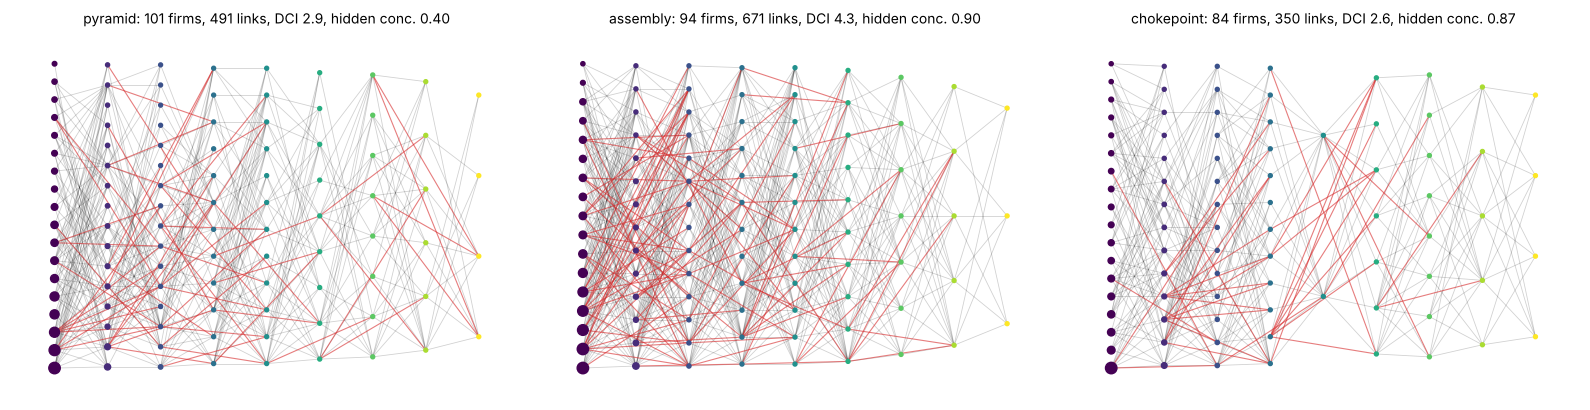
\includegraphics[width=\textwidth]{fig_atlas.png}
\caption{Network atlas: one pilot network per family, laid out by tier (raw materials left, OEMs right). Node size is throughput; red links are closure (tier-skipping) sourcing.}
\label{fig:atlas}
\end{figure*}

\begin{table}[t]
\caption{Mean fingerprint per family (pilot, training-scale and larger networks).}
\label{tab:fp}
\centering\small
\begin{tabular}{lrrr}
\toprule
 & Pyramid & Assembly & Chokepoint \\
\midrule
Firms & \pilot{130} & \pilot{115} & \pilot{103} \\
Links & \pilot{734} & \pilot{851} & \pilot{467} \\
Max out-degree & \pilot{16.1} & \pilot{22.0} & \pilot{15.7} \\
Assortativity & \pilot{$-0.01$} & \pilot{0.00} & \pilot{$-0.16$} \\
Degree of commonality & \pilot{2.89} & \pilot{4.43} & \pilot{2.56} \\
Dual-sourcing share & \pilot{0.25} & \pilot{0.20} & \pilot{0.23} \\
Hidden concentration & \pilot{0.73} & \pilot{0.74} & \pilot{0.72} \\
$z$ shared supplier & \pilot{10.0} & \pilot{9.1} & \pilot{5.7} \\
$z$ transitive triangle & \pilot{10.7} & \pilot{15.5} & \pilot{11.0} \\
\bottomrule
\end{tabular}
\end{table}

\subsection{Anatomy of cascades (H1)}
\pilot{22.1\%} of firm--scenario pairs suffer a service failure, but only \pilot{20\%} of failures are downstream of the disrupted firm (Fig.~\ref{fig:anatomy}). Downstream failures fade within about three hops (failure rate \pilot{0.38, 0.22, 0.05} at hops 1--3) as stock buffers absorb the shortage. Lateral failures reach up to \pilot{five} hops and are split between supply-caused and overload-caused parents (\pilot{2\,831} vs \pilot{1\,593}): alternative suppliers are overloaded by rerouted orders and pass the shortage to their other customers. Upstream, \pilot{31.2\%} of ancestors fail -- mostly through the recovery surge, when the disrupted firm restarts and orders a burst its suppliers cannot meet \citep{Li2021}. Fig.~\ref{fig:propagation} follows one cascade. Firm \pilot{34} (T5) of a chokepoint network is down for \pilot{56} days, and its buyers detect the outage and reroute after \pilot{7.7} days. The first failures are \emph{lateral}: on days \pilot{17} and \pilot{20}, two alternative suppliers of the disrupted firm -- they share a sourcing group with it -- fail because the rerouted orders of a common T4 buyer exceed their capacity (overload-caused links, panel e). The \emph{downstream} shortage arrives only after stocks are used up. It reaches that T4 buyer on day \pilot{26}, T3 from day \pilot{34} (most between days \pilot{50} and \pilot{72}), T2 on days \pilot{55--62} and T1 on days \pilot{83--86}, and never reaches the OEMs. \emph{Upstream}, the disrupted firm's suppliers change their orders without failing (transmitters, days \pilot{19--36}), and raw-material firms further up fail from overload. Failures keep rising after the restart on day \pilot{56}: the downstream wave is still travelling, and catch-up orders overload suppliers (panel f). In total \pilot{51} of the \pilot{81} other firms fail. On day \pilot{151}, \pilot{20} are still in failure and \pilot{31} have recovered (panel d). Diamonds weaken dual sourcing: downstream firms exposed through a diamond fail in \pilot{10.8\%} ($\pm\pilot{2.6}$) of cases, more than firms with an independent alternative (\pilot{9.2\%} $\pm\pilot{1.2}$) but fewer than single-sourced firms (\pilot{15.6\%}). In the pilot, diamonds therefore \emph{erode} rather than cancel the protection of dual sourcing. \todo{Confirm with the full run.}

\begin{figure*}[t]
\centering
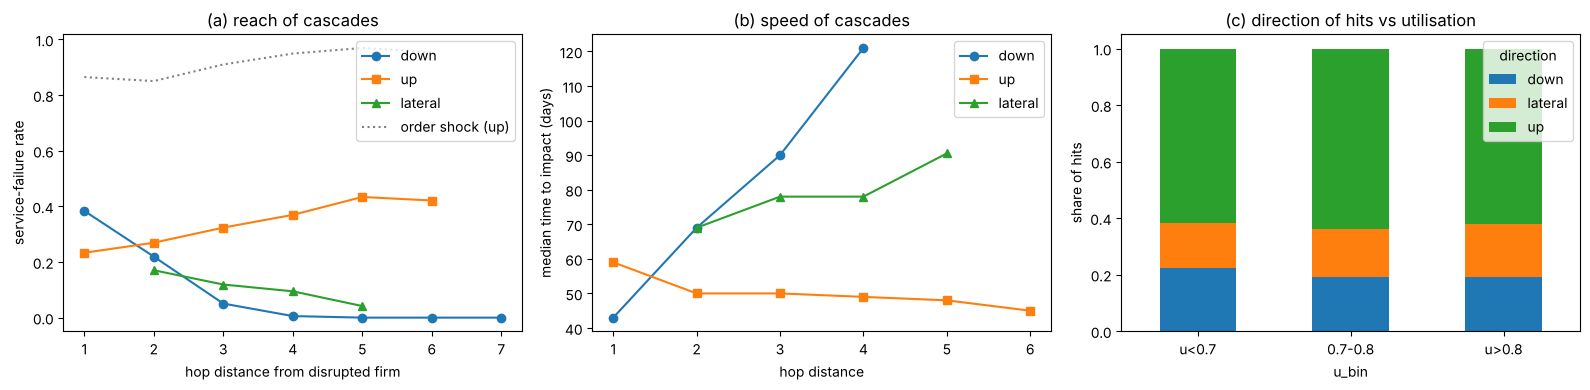
\includegraphics[width=\textwidth]{fig_anatomy.png}
\caption{Cascade anatomy (pilot). (a) Service-failure rate by hop distance and direction; dotted: order shocks travelling upstream. (b) Median time to impact. (c) Direction of failures by utilisation.}
\label{fig:anatomy}
\end{figure*}

\begin{figure*}[t]
\centering
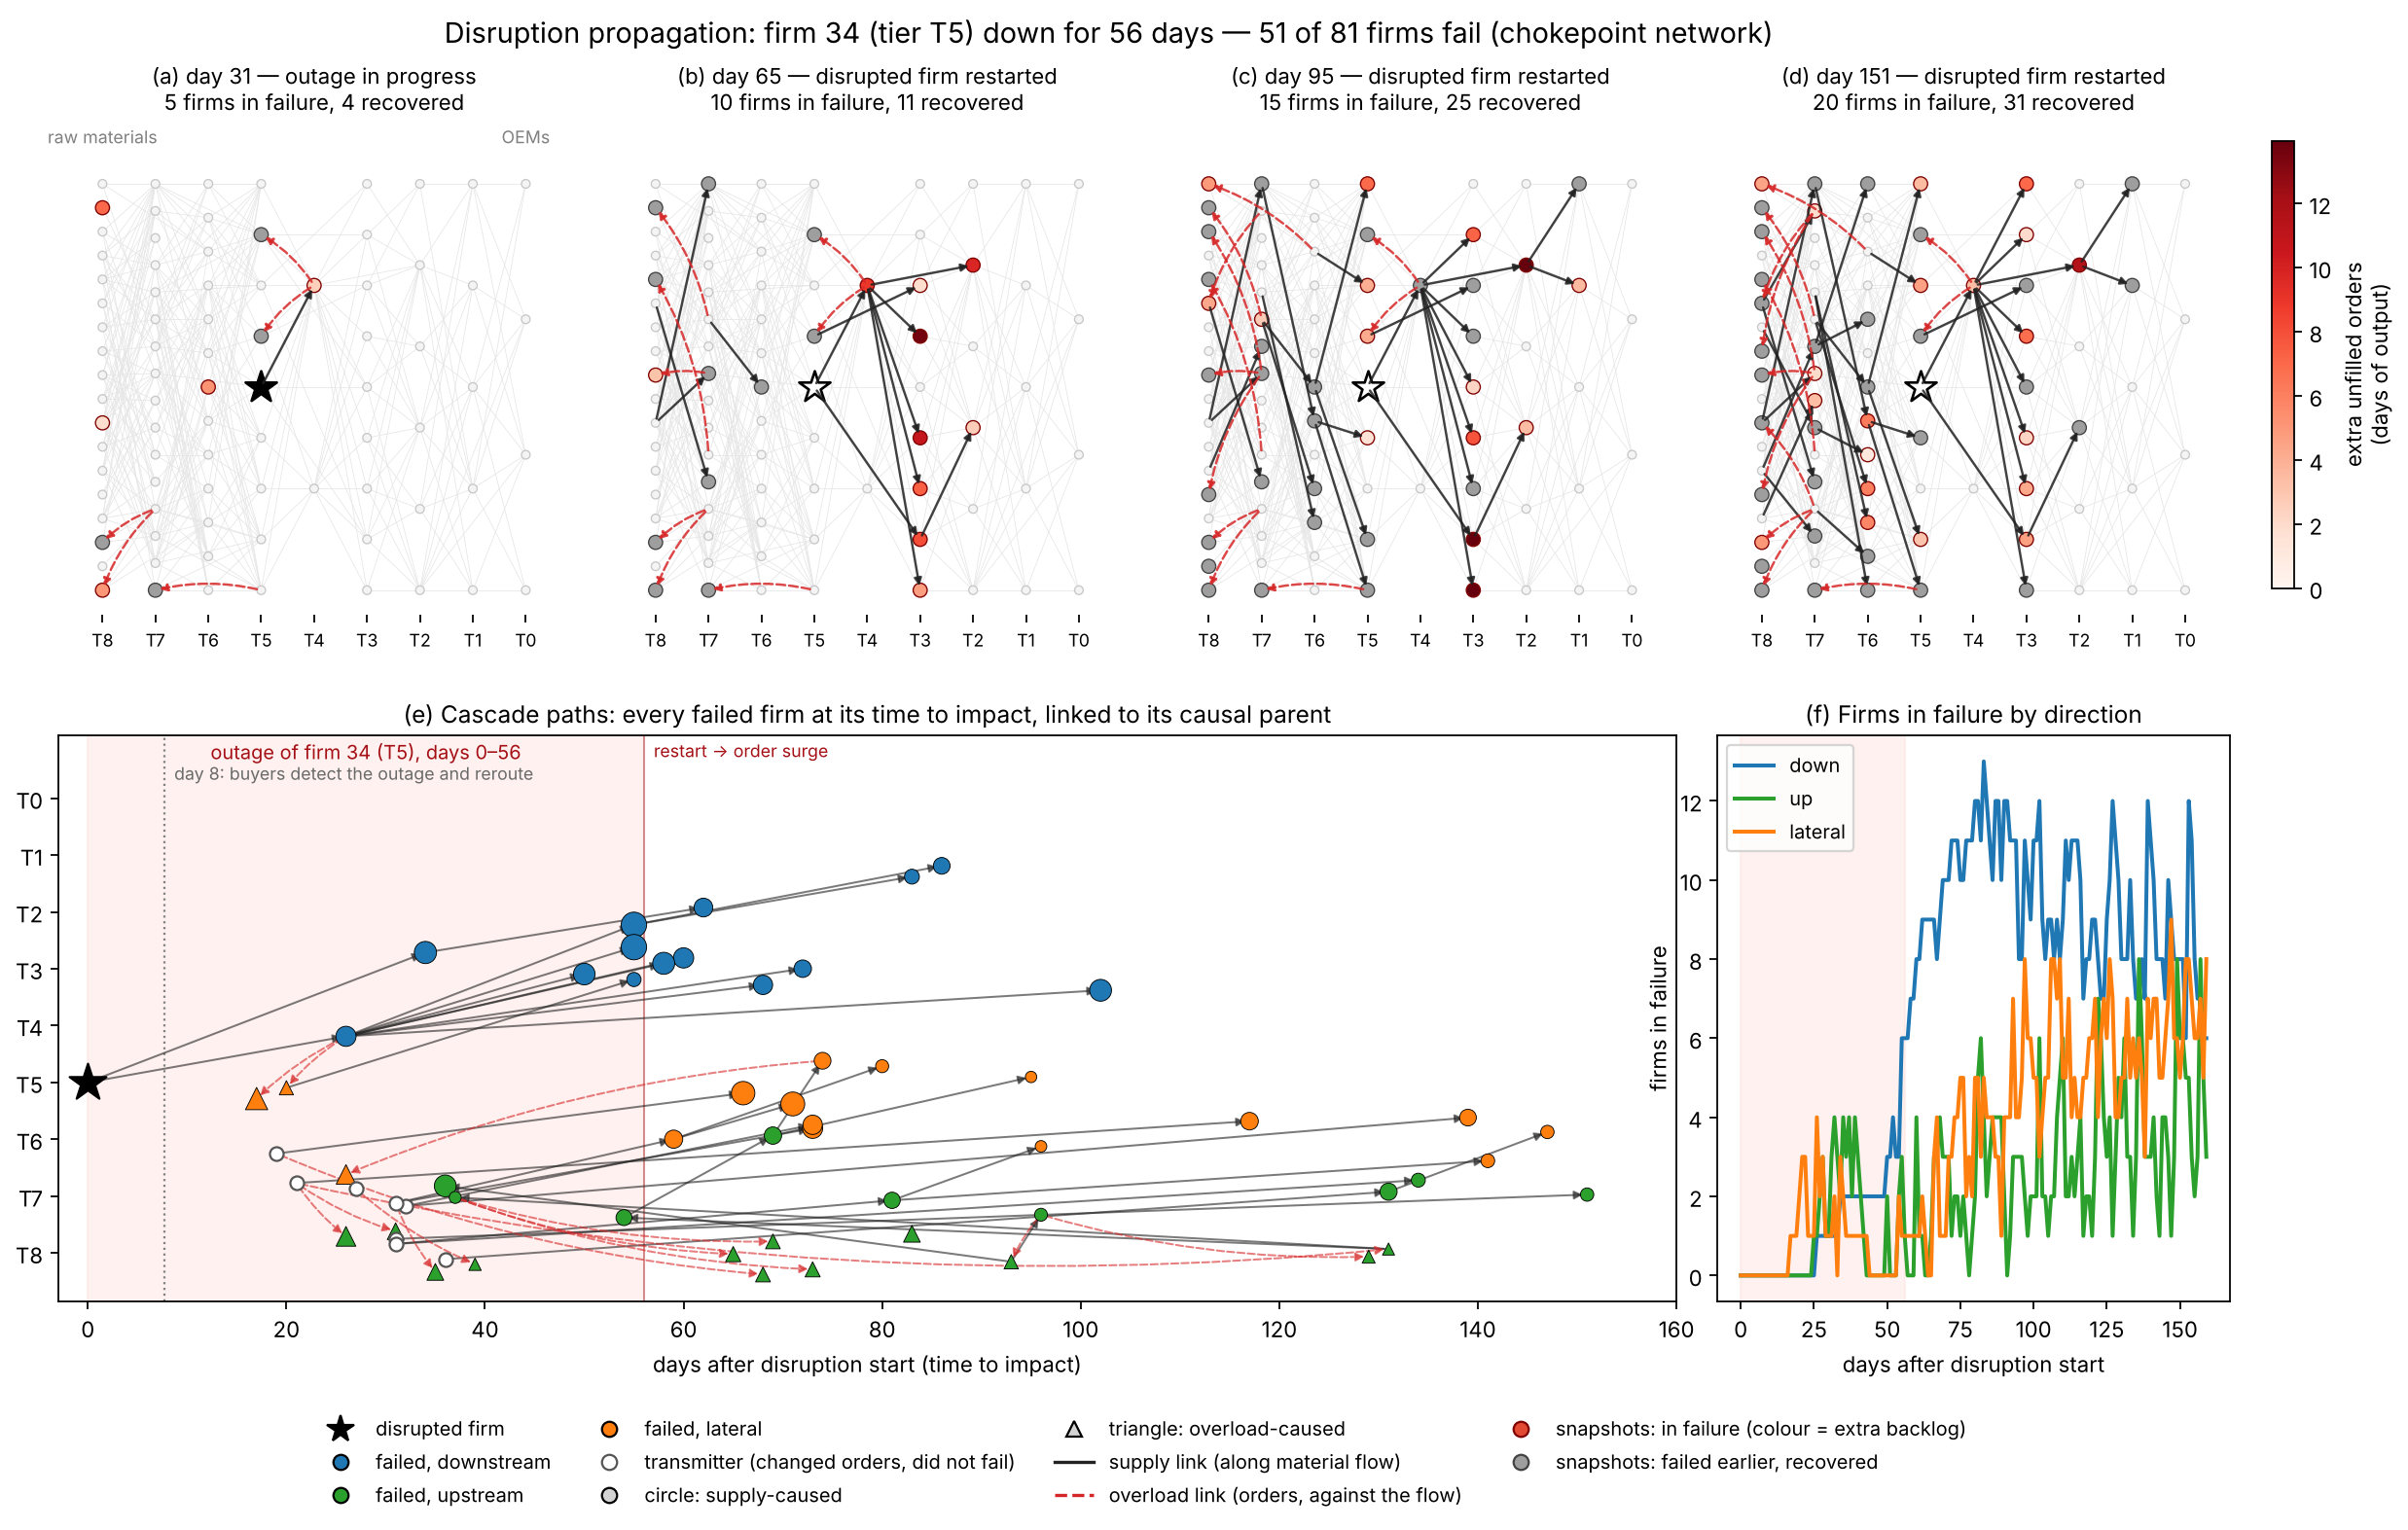
\includegraphics[width=\textwidth]{fig_propagation.png}
\caption{How one disruption propagates (pilot): firm \pilot{34} (tier T5) of a chokepoint network is down for \pilot{56} days.
(a)--(d) The whole network at the days by which 10\%, 40\%, 75\% and all failures have started; raw materials left, OEMs right. Red firms are in failure (shade = extra unfilled orders, in days of output); grey firms failed earlier and have recovered. Arrows are the causal-parent links active so far: solid = supply-caused, along the material flow; dashed red = overload-caused, orders travelling against the flow. The star is the disrupted firm (black while down).
(e) Cascade paths: every failed firm at (time to impact, tier), linked to its causal parent $p(f)$. Colour = direction, circle/triangle = supply/overload-caused, size = severity. Hollow circles are transmitters (firms that changed their orders without failing). Shaded: the outage; dotted: detection and rerouting.
(f) Number of firms in failure by direction.}
\label{fig:propagation}
\end{figure*}

\subsection{What topology-based rules miss (H2)}
Both rules only predict downstream failures. The cascade rule recovers \pilot{94.2\%} of downstream failures but only \pilot{18.9\%} of all failures (precision \pilot{0.44}), and its timing error on correctly predicted failures is \pilot{26.2} days; reachability recovers all downstream failures with precision \pilot{0.15} and a timing error of \pilot{57.8} days.

\subsection{GNN prediction (H3)}
Table~\ref{tab:gnn} compares models on unseen networks at training scale and on larger unseen networks. The AND/OR-GNN has the highest AUPRC and F1 on both. Its timing error matches the generic GNN on test networks and is lower on larger ones. It leads in all three directions (Fig.~\ref{fig:gnn}b), is highest or level at every hop distance (Fig.~\ref{fig:gnn}a), and does not lose accuracy on larger networks (Fig.~\ref{fig:gnn}c). One forward pass takes \pilot{22.2} ms against \pilot{150} ms for one DES run of the same network.

\begin{table}[t]
\caption{Failure prediction on unseen networks (pilot, one seed). $\tau$: mean absolute error in days on correctly predicted failures.}
\label{tab:gnn}
\centering\small
\setlength{\tabcolsep}{4pt}
\begin{tabular}{lccc|ccc}
\toprule
 & \multicolumn{3}{c|}{Test (same scale)} & \multicolumn{3}{c}{Larger networks} \\
Model & AUPRC & F1 & $\tau$ & AUPRC & F1 & $\tau$ \\
\midrule
AND/OR-GNN & \pilot{.73} & \pilot{.63} & \pilot{20.6} & \pilot{.70} & \pilot{.64} & \pilot{24.4} \\
Generic GNN & \pilot{.46} & \pilot{.57} & \pilot{20.5} & \pilot{.52} & \pilot{.57} & \pilot{25.4} \\
Feature MLP & \pilot{.44} & \pilot{.45} & \pilot{23.1} & \pilot{.51} & \pilot{.48} & \pilot{25.9} \\
Cascade rule & -- & \pilot{.31} & \pilot{21.1} & -- & \pilot{.24} & \pilot{28.5} \\
Reachability & -- & \pilot{.18} & \pilot{51.5} & -- & \pilot{.15} & \pilot{61.0} \\
\bottomrule
\end{tabular}
\end{table}

\begin{figure*}[t]
\centering
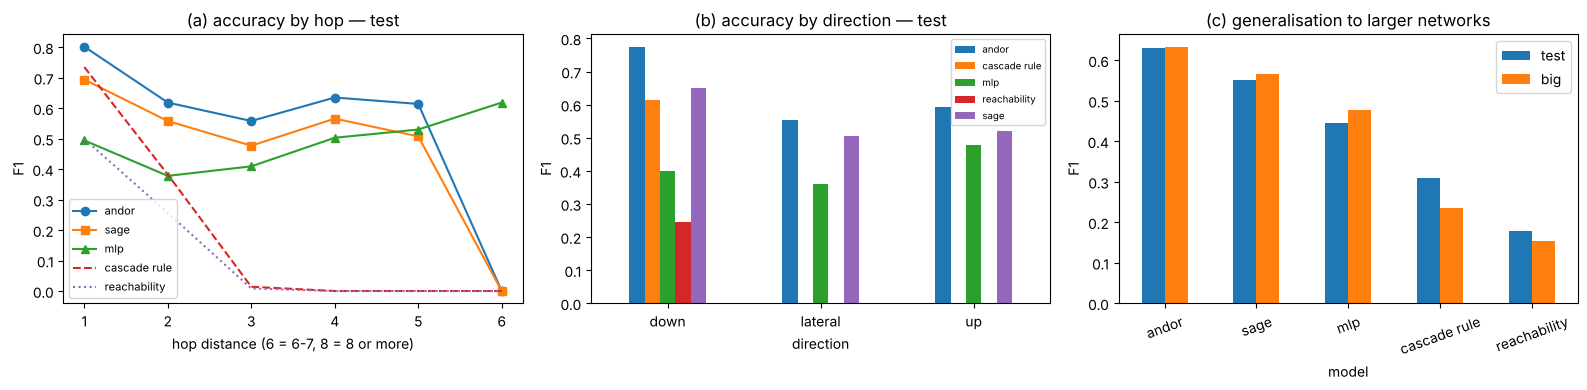
\includegraphics[width=\textwidth]{fig_gnn.png}
\caption{Failure prediction on test networks (pilot). (a) F1 by hop distance. (b) F1 by direction. (c) F1 on test vs larger networks.}
\label{fig:gnn}
\end{figure*}

%% ----------------------------------------------------------------------------
\section{Conclusion}

On product-integrated multi-tier networks, most service failures caused by a disruption are not downstream of it: they reach alternative suppliers through rerouted orders and reach upstream suppliers through the recovery surge. Cascade rules that follow the material flow cannot see them. A GNN whose message passing mirrors the AND logic of the BOM and the OR logic of multi-sourcing learns these cascades from discrete-event ground truth and transfers to unseen and larger networks, at a small fraction of the simulation cost. Limitations: the pilot is small and uses one training seed; networks are synthetic; and the model is deterministic, with a single disruption at a time. Future work will run the full study, add real topologies and stochastic demand, and predict the causal parent -- the cascade path itself.

%% ----------------------------------------------------------------------------
\begin{ack}
\todo{Funding acknowledgement, e.g. Horizon Europe project ACCURATE (GA 101138269), if applicable.}
\end{ack}

%% References: verify every entry before submission.
\begin{thebibliography}{99}

\bibitem[Ang et~al.(2017)]{Ang2017}
Ang, E., Iancu, D.A., and Swinney, R. (2017).
\newblock Disruption risk and optimal sourcing in multitier supply networks.
\newblock \emph{Management Science}, 63(8), 2397--2419.

\bibitem[Atalay et~al.(2011)]{Atalay2011}
Atalay, E., Horta\c{c}su, A., Roberts, J., and Syverson, C. (2011).
\newblock Network structure of production.
\newblock \emph{Proceedings of the National Academy of Sciences}, 108(13), 5199--5202.

\bibitem[Choi and Wu(2009)]{ChoiWu2009}
Choi, T.Y. and Wu, Z. (2009).
\newblock Triads in supply networks: theorizing buyer--supplier--supplier relationships.
\newblock \emph{Journal of Supply Chain Management}, 45(1), 8--25.

\bibitem[Collier(1981)]{Collier1981}
Collier, D.A. (1981).
\newblock The measurement and operating benefits of component part commonality.
\newblock \emph{Decision Sciences}, 12(1), 85--96.

\bibitem[Dolgui et~al.(2018)]{Dolgui2018}
Dolgui, A., Ivanov, D., and Sokolov, B. (2018).
\newblock Ripple effect in the supply chain: an analysis and recent literature.
\newblock \emph{International Journal of Production Research}, 56(1--2), 414--430.

\bibitem[Hamilton et~al.(2017)]{Hamilton2017}
Hamilton, W.L., Ying, R., and Leskovec, J. (2017).
\newblock Inductive representation learning on large graphs.
\newblock In \emph{Advances in Neural Information Processing Systems 30}.

\bibitem[Ivanov et~al.(2014)]{Ivanov2014}
Ivanov, D., Sokolov, B., and Dolgui, A. (2014).
\newblock The ripple effect in supply chains: trade-off `efficiency--flexibility--resilience' in disruption management.
\newblock \emph{International Journal of Production Research}, 52(7), 2154--2172.

\bibitem[Kosasih and Brintrup(2022)]{Kosasih2022}
Kosasih, E.E. and Brintrup, A. (2022).
\newblock A machine learning approach for predicting hidden links in supply chain with graph neural networks.
\newblock \emph{International Journal of Production Research}, 60(17), 5380--5393.

\bibitem[Li et~al.(2021)]{Li2021}
Li, Y., Chen, K., Collignon, S., and Ivanov, D. (2021).
\newblock Ripple effect in the supply chain network: forward and backward disruption propagation, network health and firm vulnerability.
\newblock \emph{European Journal of Operational Research}, 291(3), 1117--1131.

\bibitem[Milo et~al.(2002)]{Milo2002}
Milo, R., Shen-Orr, S., Itzkovitz, S., Kashtan, N., Chklovskii, D., and Alon, U. (2002).
\newblock Network motifs: simple building blocks of complex networks.
\newblock \emph{Science}, 298(5594), 824--827.

\bibitem[Simchi-Levi et~al.(2015)]{SimchiLevi2015}
Simchi-Levi, D., Schmidt, W., Wei, Y., Zhang, P.Y., Combs, K., Ge, Y., Gusikhin, O., Sanders, M., and Zhang, D. (2015).
\newblock Identifying risks and mitigating disruptions in the automotive supply chain.
\newblock \emph{Interfaces}, 45(5), 375--390.

\bibitem[Zhao et~al.(2019)]{Zhao2019}
Zhao, K., Zuo, Z., and Blackhurst, J.V. (2019).
\newblock Modelling supply chain adaptation for disruptions: an empirically grounded complex adaptive systems approach.
\newblock \emph{Journal of Operations Management}, 65(2), 190--212.

\end{thebibliography}

%% ============================================================================
\appendix
\section{Reproducibility specification}
\label{app:repro}

This appendix, with the reference implementation, fixes every quantity needed to regenerate the networks, the ground truth and the models. Where the text and the code could be read differently, the code is normative.

\subsection{Code, environment and verification}
\begin{itemize}
\item \textbf{Code.} Notebook \texttt{scsim/scripts/research/ripple/incom2027\_cascade.ipynb} in the SuReSuite repository, commit \texttt{\nbcommit}. It is self-contained: Stage~1 generation, Stage~2 simulation, Stage~3 labels and baselines, Stage~4 GNN.
\item \textbf{Environment.} Python 3.13.16; numpy 2.5.3; pandas 3.0.5; networkx 3.7; scikit-learn 1.9.1; scipy 1.18.1; matplotlib 3.11.2; torch 2.14.1, CPU only; Linux x86\_64. The versions are pinned in \texttt{requirements.txt} next to the notebook.
\item \textbf{Run.} Set the environment variable \texttt{RIPPLE\_MODE} to \texttt{quick} (pilot) or \texttt{incom} (full study) and execute all cells in order. The pilot takes about 13~minutes on four CPU cores.
\item \textbf{Verification.} The notebook prints two SHA-256 digests.
  \begin{itemize}
  \item The \emph{network digest} covers, for every network in order: firm tiers, portfolios, BOMs, sourcing sets, lead times, rates $x_{f,i}$, capacities, base stocks, FG targets and $\delta$.
  \item The \emph{label digest} covers, for every scenario in order: network, target, duration, and per firm the failure flag, $\tau_f$, $\sigma_f$ and $p(f)$.
  \end{itemize}
  For the pilot they are \texttt{\netdigest} and \texttt{\labeldigest}. A run that prints both digests reproduced the networks and the ground truth bit for bit. Two independent executions gave identical digests.
\item \textbf{Bit-exactness.} The simulation is deterministic and uses IEEE double precision throughout. NumPy random streams are reproducible for a fixed NumPy version, which is why versions are pinned. GNN training runs with \texttt{torch.use\_deterministic\_algorithms(True)}; it is repeatable on the same hardware and thread count, but other CPUs may differ in the last bits, which moves model metrics at most in the third decimal.
\end{itemize}

\subsection{Seeds and random streams}
All random draws use NumPy \texttt{Generator}s (PCG64). Uniform integers $\mathcal{U}\{a,\dots,b\}$ are \texttt{integers(a, b+1)}; uniform reals are \texttt{uniform} or \texttt{random}; choices are \texttt{choice}.
\begin{center}\footnotesize
\begin{tabular}{p{2.6cm}p{5.2cm}}
\toprule
Stream & Seed and use \\
\midrule
Master & 2027: \texttt{np.random.seed}, \texttt{random.seed}, \texttt{torch.manual\_seed} (no draws are taken from these global streams) \\
Network set & \texttt{Generator(2027)}: Latin hypercubes, splits, network seeds $\omega_n$ (Sec.~\ref{app:set}) \\
Structure & \texttt{Generator}($\omega_n$): every draw of Algorithm~\ref{alg:gen}, steps 1--5, in the order of Sec.~\ref{app:gen} \\
Quantities & \texttt{Generator}($\omega_n+7$): lead times (links in lexicographic order of (supplier, buyer)), then $u_f$, then $s_f$, then $s^{FG}_f$ (firms in index order) \\
Demand & \texttt{Generator}($1000\,\omega_n+i$).\texttt{uniform(5,20)} for end item $i$ \\
Targets & \texttt{Generator}($\omega_n+99$): disrupted firms per tier \\
Triad null & \texttt{Generator(2028)}, shared by the atlas networks in network order \\
GNN & \texttt{torch.manual\_seed(0)} and \texttt{Generator(0)} (batch order), reset for every model \\
\bottomrule
\end{tabular}
\end{center}
If a generated network fails the structural checks, its seed is increased by one and generation is repeated, at most five times.

\subsection{Construction of the network set}
\label{app:set}
The families are processed in the order pyramid, assembly, chokepoint. For each family, with $n=n_{\mathrm{s}}+n_{\mathrm{b}}$ networks ($n_{\mathrm{s}}$ at training scale, $n_{\mathrm{b}}$ larger), the stream draws:
\begin{enumerate}
\item a Latin hypercube. For each factor in the order $u,\rho,\alpha,\beta,\kappa,\tau,\tau_d,s,s^{FG},\delta$, draw a permutation $\pi$ of $\{0,\dots,n-1\}$ and $U_r\sim\mathcal{U}[0,1)$; row $r$ receives $\mathrm{lo}+(\pi_r+U_r)/n\cdot(\mathrm{hi}-\mathrm{lo})$.
\item a permutation of the $n_{\mathrm{s}}$ training-scale rows. The first $\mathrm{round}(0.7n_{\mathrm{s}})$ in that order go to training, the next $\max(1,\mathrm{round}(0.15n_{\mathrm{s}}))$ to validation, the rest to test. Rows $n_{\mathrm{s}},\dots,n-1$ are the larger networks.
\item one seed $\omega_n\sim\mathcal{U}\{0,\dots,10^9-1\}$ per row, in row order.
\end{enumerate}
Item counts per tier are $\max(2,\mathrm{round}(w_k\cdot\mathrm{scale}))$, with Python rounding (ties to even). The chokepoint tier is fixed at 3 items and is not scaled. The run settings are in Table~\ref{tab:runs}.

\begin{table}[h]
\caption{Run settings.}
\label{tab:runs}
\centering\footnotesize
\begin{tabular}{lcc}
\toprule
Setting & Pilot (\texttt{quick}) & Full (\texttt{incom}) \\
\midrule
networks per family ($n_{\mathrm{s}}$+$n_{\mathrm{b}}$) & 8+3 & 200+30 \\
train/val/test networks per family & 6/1/1 & 140/30/30 \\
scale (training / larger) & 0.5 / 1.0 & 1.0 / 2.0 \\
targets per tier (T1--T8) & 2 & 4 \\
durations $D$ (days) & 21, 56 & 14, 28, 56, 84 \\
warm-up $W$ / horizon $H$ (days) & 120 / 160 & 150 / 240 \\
null samples (atlas networks) & 10 & 20 \\
GNN width $d_h$ / epochs & 64 / 25 & 96 / 80 \\
\bottomrule
\end{tabular}
\end{table}

\subsection{Generator: exact rules}
\label{app:gen}
\begin{itemize}
\item \emph{Items.} Items are numbered consecutively, tier by tier from T0. The number of platforms is $P=\min(P_{\mathrm{tmpl}},w_0)$. The $j$-th end item gets platform $j\bmod P$; every other item gets one drawn from $\mathcal{U}\{0,\dots,P-1\}$, one draw per item in index order (end items included, then overwritten).
\item \emph{BOM.} For tiers $k=0..7$ and items $i$ in index order: $m_i=\min(\mathcal{U}\{m_{\min},\dots,m_{\max}\},w_{k+1})$. The $m_i$ components are drawn by one \texttt{choice} without replacement over the tier-$(k{+}1)$ items, with probabilities $\propto(\mathrm{use}_j+1)^{\alpha_b}\cdot[\pi(j){=}\pi(i)\ ?\ 1:\mu]$. Then, for each drawn component in draw order, $a_{ij}\sim\mathcal{U}\{1,2,3\}$ and $\mathrm{use}_j\mathrel{+}=1$.
\item \emph{Repair.} For tiers $k=1..8$ and items in index order, an item with $\mathrm{use}_j=0$ is added to the BOM of a parent drawn uniformly from the same-platform items of tier $k-1$ (all items of $k-1$ if there are none), with $a\sim\mathcal{U}\{1,2,3\}$.
\item \emph{Closure.} For tiers $k=0..6$ and items $i$ in index order; for each regular component $j$ of $i$ in insertion order; for each regular component $l$ of $j$ in insertion order: if $l\notin\mathrm{BOM}(i)$, draw $U$, and if $U<\tau$ add $l$ with $a_{il}=1$.
\item \emph{Firms.} For each tier, platforms are visited in a random permutation. Within a platform the items are put in a random permutation and cut into consecutive portfolios, each of size $\mathcal{U}\{p_{\min},\dots,p_{\max}\}$ (the last may be smaller). Firms are numbered in creation order.
\item \emph{Extra producers.} For each item of the tier in index order, two attempts. Let $A$ be the firms of the tier that do not yet produce it. If $A\neq\emptyset$, draw $U$; if $U<q$, choose uniformly from the same-platform firms in $A$ if there are any and a second draw is $<0.8$, otherwise uniformly from $A$.
\item \emph{Sourcing order.} Tiers $k=0..7$. The firms of the tier are visited in a random permutation, and each firm's regular components in ascending index. ``Earlier buyers'' of $c$ are the groups of $c$ already created, and $\mathrm{buyers}(s)$ counts every group that already includes $s$.
\item \emph{Sourcing rule for group $(f,c)$.}
  \begin{itemize}
  \item $\Sigma$ is the union of the supplier sets of $c$ held by $f$'s co-sources.
  \item If $\Sigma\neq\emptyset$: draw $U$; if $U<\kappa$, the first supplier is chosen uniformly from $\Sigma$ in ascending order; otherwise, if $\mathrm{Prod}(c)\setminus\Sigma\neq\emptyset$, the set $\Sigma$ is excluded.
  \item If no supplier has been chosen and $c$ has earlier buyers: draw $U$; if $U<\beta$, take the most frequent first supplier among them, excluding $\Sigma$ if excluded, with ties broken by the lowest firm index. If none remains, fall through to the next rule.
  \item Otherwise, draw from $\mathrm{Prod}(c)$ minus the excluded set with probability $\propto(\mathrm{buyers}(s)+1)^{\alpha}$.
  \item Second source: if $|\mathrm{Prod}(c)|\ge2$, draw $U$; if $U<\rho$, add a second producer by the same weights, excluding only the first.
  \end{itemize}
\item \emph{Coverage and co-sources.} After each tier $k$, every item $c$ of tier $k{+}1$ is visited in index order. Each producer of $c$ that appears in none of $c$'s groups is appended to one of those groups, chosen uniformly. Then every pair of suppliers in the same group is recorded as co-sources.
\item \emph{Closure sourcing.} Firms in index order, closure components in ascending index. Draw $U$; if $U<\tau_d$, choose uniformly (ascending order) among the suppliers that $f$'s regular suppliers use for $c$, if any. Otherwise use the hub rule. Closure groups have one supplier.
\item \emph{Final coverage.} Every non-end item is visited in index order; each of its producers that appears in none of its groups is appended to a uniformly chosen group of that item.
\end{itemize}

\subsection{Quantities: exact rules}
\begin{itemize}
\item \emph{Rates.} $x_{f,i}=d_i/|\mathrm{Prod}(i)|$ for end items. Then, for tiers $k=0..8$: for every firm of tier $k$ and every item in its portfolio, $n_{(f,c)}\mathrel{+}=x_{f,i}\,a_{ic}$; after the tier, every group $(f,c)$ of the tier adds $n_{(f,c)}/|S_{(f,c)}|$ to $x_{s,c}$ for each $s\in S_{(f,c)}$.
\item \emph{Pruning.} Pairs with $x_{f,i}\le10^{-9}$ and groups with $n_g\le10^{-9}$ are dropped (none occur).
\item \emph{Ordering.} Groups are ordered by (tier of $f$, $f$, $c$) and links lexicographically. The firm graph's adjacency follows this order, so predecessor and successor lists are in ascending firm index.
\item \emph{Parameters.} $L_{sf}\sim\mathcal{U}\{2,\dots,3+k(s)\}$; $u_f=\mathrm{clip}(u+\mathcal{U}[-0.05,0.05],0.3,0.97)$; $C_f=x_f/u_f$; $s_f=s\cdot\mathcal{U}[0.5,1.5]$; $s^{FG}_f=s^{FG}\cdot\mathcal{U}[0.5,1.5]$.
\item \emph{Stock levels.} $L_g=\max_{s\in S_g}L_{sf}$; $S_g=n_g(L_g+14+s_f)$; $Q_g=7n_g$; $S^{FG}_{f,i}=x_{f,i}(7+s^{FG}_f)$; $Q_{f,i}=7x_{f,i}$.
\end{itemize}

\subsection{Simulation: exact rules}
\begin{itemize}
\item \emph{Event list.} A binary heap keyed by (time, priority, creation counter). Priorities: control 0, arrival 1, completion 2, market order 3, sampling 9. The creation counter increases by one per scheduled event.
\item \emph{Market orders.} One per OEM item at $t=0$, then every 1.0 day.
\item \emph{Immediacy.} Orders have no information delay. Placing an order appends it to the supplier's queue and immediately calls ``try to ship'' and ``try to produce'' at that supplier, within the same event.
\item \emph{Tolerance.} Stock comparisons use a tolerance of $10^{-9}$.
\item \emph{Production choice.} Items are visited in portfolio order. An item is chosen only if its gap exceeds the best so far by more than $10^{-9}$, so ties go to the earlier item.
\item \emph{During an outage.} A lot already in progress completes. At restart the firm first tries to ship each item in portfolio order, then tries to produce.
\item \emph{Rotation.} Each group keeps a counter of orders placed. The supplier is the $(\text{counter} \bmod |A_g|)$-th element of the active list $A_g$ (suppliers not excluded, in $S_g$ order; all of $S_g$ if every supplier is excluded). Exclusion is global: every buyer of $v$ stops ordering from it at $t_0+\delta$.
\item \emph{Branching.} The warm-up processes all events with $t\le W$; the state is then deep-copied.
  \begin{itemize}
  \item A disrupted branch schedules, in this order: start ($t_0$), end ($t_0+D$), exclude ($t_0+\delta$), include ($t_0+D+\delta$).
  \item The clean branch schedules four no-op control events at $t_0$, which keeps the creation counters aligned.
  \item Both schedule the first sampling event at $t_0+0.5$ and process all events with $t\le t_0+H$.
  \end{itemize}
\item \emph{Validation.}
  \begin{itemize}
  \item Fill rate: market units shipped divided by market units ordered between the first and last samples.
  \item Stability: with $b(k)=\sum_f B_f(k)/x_f$, the mean of $b$ over the second half of the samples may exceed the mean over the first half by at most $0.1\times$ the first-half mean $+2$.
  \end{itemize}
\end{itemize}

\subsection{Labels and baselines: exact rules}
\begin{itemize}
\item \emph{Time index.} Sample $k$ (taken at $t_0+k+0.5$) is day $k$. $\tau_f$ is the smallest $k$ with $\Delta_f(k),\dots,\Delta_f(k+P-1)\ge\theta$; firms without such a $k$ have no $\tau_f$. The disrupted firm is excluded from every label set and metric.
\item \emph{Parent ties.} Ties in $p(f)$ go to the lowest firm index. Planned flows below $10^{-9}$ are floored at $10^{-9}$.
\item \emph{Hop distance.} Breadth-first search on the undirected firm graph; unreachable firms get 99.
\item \emph{Reachability.} $\tau$ is the Dijkstra distance from $v$ on $G$ with link weights $L_{sf}$.
\item \emph{Cascade rule.} Firms are visited in \texttt{networkx.topological\_sort} order. If $D-c^{FG}_v\le0$, no firm is hit.
\item \emph{Exposure classes} (H1), for every downstream firm $f$.
  \begin{itemize}
  \item A group is \emph{exposed} if at least one of its suppliers is $v$ or downstream of $v$.
  \item $f$ is \emph{single} if some exposed group has one supplier.
  \item Otherwise it is \emph{diamond} if some exposed group has all its suppliers exposed.
  \item Otherwise it is \emph{independent dual} if it has an exposed group, and \emph{none} if it has none.
  \end{itemize}
  The 95\% interval is $\pm1.96\sqrt{\hat p(1-\hat p)/n}$.
\end{itemize}

\subsection{GNN: exact rules}
\begin{itemize}
\item \emph{MLPs.} $\mathrm{MLP}(a\to b)=\mathrm{Linear}(a,b)$--GELU--$\mathrm{Linear}(b,b)$, with PyTorch default initialisation.
\item \emph{Modules.}
  \begin{itemize}
  \item Firm encoder: $\mathrm{MLP}(20\to d_h)$; $\mathrm{MLP}(24\to d_h)$ for the feature MLP.
  \item Group encoder $\phi_0$: $\mathrm{MLP}(4\to d_h)$.
  \item Per AND/OR layer: $\phi_1,\phi_4,\phi_5$: $\mathrm{MLP}(d_h{+}1\to d_h)$; $\phi_2$: $\mathrm{MLP}(4d_h\to d_h)$; $\phi_3$: $\mathrm{MLP}(2d_h{+}1\to d_h)$; $\phi_6$: $\mathrm{MLP}(7d_h\to d_h)$; LayerNorm($d_h$).
  \item Per generic layer: $\phi_4,\phi_5$ as above, $\phi_6$: $\mathrm{MLP}(3d_h\to d_h)$.
  \item Head: $\mathrm{MLP}(d_h\to3)$.
  \item Aggregations over an empty set return 0 (e.g.\ raw-material firms have no groups).
  \end{itemize}
\item \emph{Features.} Firm features are in this order: tier one-hot (9); $u_f$; $\log(1+x_f)/5$; $(s^{FG}_f+3.5)/10$; $|I_f|/4$; $\log(1+\text{out-degree})/3$; $\log(1+\text{in-degree})/3$; share of $f$'s groups with $|S_g|>1$ (0 if none); $(s_f+3.5)/10$; mean lead time over all incoming links $/10$ (0 if none); target flag; $D/\max D$. The feature MLP appends $\min(\text{hop},12)/12$ and down/up/lateral indicators.
\item \emph{Targets.} Failure $y_f\in\{0,1\}$; $\tau_f/H$ (0 where $y_f=0$, not used); $\log(1+\sigma_f)$.
\item \emph{Batching.} Scenarios are concatenated as disjoint graphs with index offsets.
\item \emph{Training loop.} Per epoch:
  \begin{itemize}
  \item permute the training scenarios with \texttt{Generator(0)}, which is advanced across epochs;
  \item for each batch of 16 in that order: loss, backward pass, gradient-norm clipping at 1.0, AdamW step;
  \item after the epoch: one cosine-annealing step ($T_{\max}$ = epochs, $\eta_{\min}=0$), then predict the validation scenarios in batches of 32 and compute the AUPRC over non-target firms;
  \item keep the state if the AUPRC strictly improves.
  \end{itemize}
  The Huber loss on severity uses $\delta=1$. The positive weight is computed once from the training labels of non-target firms.
\item \emph{Threshold.} $t^\ast$ is the first maximiser of validation F1 over $\{0.05,0.10,\dots,0.95\}$; a firm is predicted to fail if its probability exceeds $t^\ast$.
\item \emph{Metrics.} scikit-learn \texttt{average\_precision\_score}, \texttt{f1\_score}, \texttt{precision\_score} and \texttt{recall\_score} over non-target firms of all scenarios of a split. The $\tau$ MAE is taken over firms with $y_f=1$ and a predicted failure. Hop bins are $\{1\},\{2\},\{3\},\{4\},\{5\},\{6,7\},\{\ge8\}$; a bin is reported only if it contains at least 5 failures.
\end{itemize}

\subsection{Fingerprints and statistics: exact rules}
\begin{itemize}
\item \emph{Degree of commonality.} The mean number of parent items over non-end items, counting regular and closure parents.
\item \emph{Producer dominance.} Over components with at least 2 producers and at least 3 (group, producer) relations: the largest producer's share of those relations.
\item \emph{Hidden concentration.} Over pairs (dual-sourced group $g$, input $l\in\mathrm{BOM}(c)$) in which every supplier of $g$ has a group for $l$ and $l$ has at least 2 producers: the share where the suppliers' sets for $l$ intersect.
\item \emph{Assortativity.} \texttt{networkx.degree\_pearson\_correlation\_coefficient} on the undirected firm graph.
\item \emph{Modularity.} With communities given by firm platforms.
\item \emph{Triad $z$-scores.} $z=(n_{\mathrm{obs}}-\bar n_{\mathrm{null}})/\mathrm{sd}_{\mathrm{null}}$, with the population standard deviation over the null samples. Each null graph places, for every tier pair, the observed number of links on distinct (supplier, buyer) cells drawn uniformly without replacement.
\item \emph{Control checks.} Spearman correlations are taken over all networks, training-scale and larger.
\end{itemize}

\end{document}
